\documentclass[tikz,border=8pt]{standalone}
\usepackage{tikz}
\usepackage{pgfplots}
\usepackage{amsmath, amssymb}

\pgfplotsset{compat=1.18}

\begin{document}

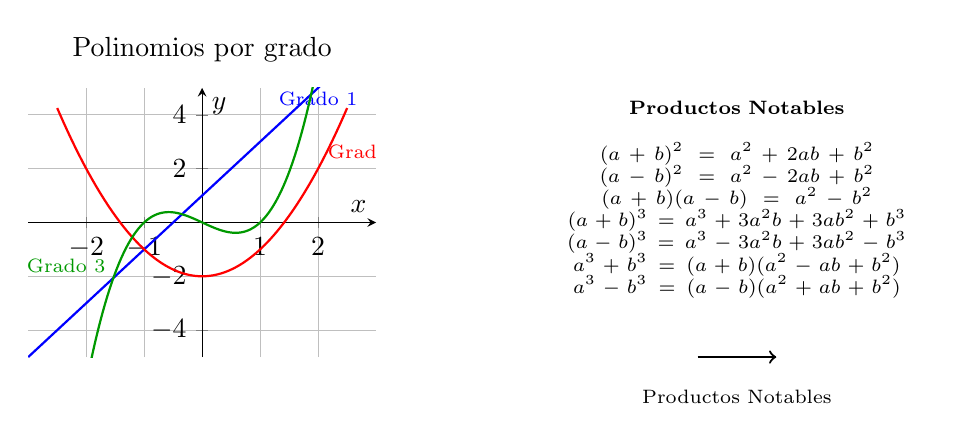
\begin{tikzpicture}[scale=1.0]

  % Gráficas de polinomios por grado
  \begin{axis}[
    axis lines = middle,
    xlabel = {$x$},
    ylabel = {$y$},
    title = {Polinomios por grado},
    xmin = -3, xmax = 3,
    ymin = -5, ymax = 5,
    xtick = {-2,-1,1,2},
    ytick = {-4,-2,2,4},
    grid = major,
    width = 6cm,
    height = 5cm,
  ]
    % Grado 1: línea recta
    \addplot[blue, thick, domain=-3:3, samples=100] {2*x + 1};
    \node[blue, above] at (axis cs:2, 4) {\scriptsize Grado 1};

    % Grado 2: parábola
    \addplot[red, thick, domain=-2.5:2.5, samples=100] {x^2 - 2};
    \node[red, above right] at (axis cs:2, 2) {\scriptsize Grado 2};

    % Grado 3: cúbica
    \addplot[green!60!black, thick, domain=-2:2, samples=100] {x^3 - x};
    \node[green!60!black, below left] at (axis cs:-1.5, -1) {\scriptsize Grado 3};
  \end{axis}

  % Árbol de productos notables (lado derecho)
  \begin{scope}[shift={(9,0)}]
    \node[align=center, text width=5cm, font=\scriptsize] at (0, 2) {
      \textbf{Productos Notables}\\
      \vspace{0.3cm}
      $(a+b)^2 = a^2+2ab+b^2$\\
      $(a-b)^2 = a^2-2ab+b^2$\\
      $(a+b)(a-b) = a^2-b^2$\\
      $(a+b)^3 = a^3+3a^2b+3ab^2+b^3$\\
      $(a-b)^3 = a^3-3a^2b+3ab^2-b^3$\\
      $a^3+b^3 = (a+b)(a^2-ab+b^2)$\\
      $a^3-b^3 = (a-b)(a^2+ab+b^2)$
    };
    \draw[thick, ->] (-0.5, 0) -- (0.5, 0);
    \node[below] at (0, -0.3) {\scriptsize Productos Notables};
  \end{scope}

\end{tikzpicture}

\end{document}
